For first-order diffraction, the position of the diffraction point can be determined in closed form.
Consider a source $\sv$, a target $\tv$, and an edge defined by its direction $\widehat{\ev}$.
For convenience, we assume the edge passes through the origin of the coordinate system, denoted by $\ov$.

According to Fermat's principle, the diffraction point $\vv$ on the edge minimizes the total path length $\sv \rightarrow \vv \rightarrow \tv$. This corresponds to minimizing the function
\begin{equation}
    \Lc \LB x \RB = \norm{\sv - \vv} + \norm{\vv - \tv}
\end{equation}
where
\begin{equation}
    \vv = x \widehat{\ev}.
\end{equation}
As shown in~\cite{4200889}, $\Lc\LB \cdot \RB$ is strictly convex and thus has a unique minimizer.

We introduce the set of vectors $\LB \widehat{\uv}_1, \widehat{\uv}_2, \widehat{\uv}_3 \RB$, where
\begin{align}
    \widehat{\uv}_1 &= \frac{\sv - \LB\widehat{\ev}\tp \sv\RB \widehat{\ev}}{\norm{\sv - \LB\widehat{\ev}\tp \sv\RB \widehat{\ev}}}\\
    \widehat{\uv}_2 &=\frac{\tv - \LB\widehat{\ev}\tp \sv\RB \widehat{\ev}}{\norm{\tv - \LB\widehat{\ev}\tp \sv\RB \widehat{\ev}}}\\
    \widehat{\uv}_3 &=
    \begin{cases}
        \widehat{\uv}_1 \times \widehat{\uv}_2 & \text{ if } \widehat{\uv}_1 \times \widehat{\uv}_2 \neq \zerov\\
        \widehat{\ev} & \text{ if } \widehat{\uv}_1 \times \widehat{\uv}_2 = \zerov
    \end{cases}
    .
\end{align}
Note that $\widehat{\uv}_3 = \pm \widehat{\ev}$, and that the source and the edge lie within the plane $\LB \ov, \widehat{\uv}_1, \widehat{\ev} \RB$.
A key observation is that rotating the target $\tv$ about the edge does not alter the path length.
Specifically, let $\Rm_{\widehat{\uv}_3} \LB \phi \RB$ denote the rotation matrix for an angle $\phi$ around the edge $\LB \ov, \widehat{\ev} \RB$. Then,
\begin{align}
    \Lc \LB x \RB &= \norm{\sv - \vv} + \norm{\vv - \tv}\\
    &= \norm{\sv - \vv} + \lVert\vv - \underbrace{\Rm_{\widehat{\uv}_3} \LB \phi \RB \tv}_{\tv'}\rVert_2\\
\end{align}
holds for any $\phi \in \RR$.
Especially, by rotating the target around the axis ($\ov, \widehat{\uv}_3$) by the angle
\begin{equation}
    \phi = \pi - \arccos \left( \widehat{\uv}_1\tp \widehat{\uv}_2 \right),
\end{equation}
the rotated target $\tv'$ is placed in the same plane $\LB \ov, \widehat{\uv}_1, \widehat{\ev} \RB$ as the source and the edge, but on the side opposite to the source with respect to the edge, as depicted in Figure~\ref{fig:diffraction-first-order}.
The rotation matrix $\Rm_{\widehat{\uv}_3} \LB \phi \RB$ is given by Rodrigues' rotation formula~\cite{Wikipedia_Rodrigues}.

\begin{figure}[ht!]
    \center
    \begin{subfigure}[b]{0.45\textwidth}
        \centering
        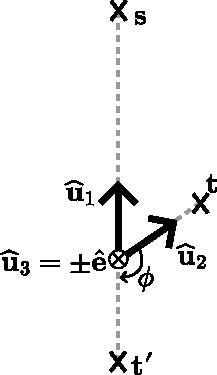
\includegraphics[width=0.35\textwidth]{figures/annex-first-order-diffraction-1.pdf}
        \caption{View in the plane $\LB \ov, \widehat{\uv}_1, \widehat{\uv}_2 \RB$, which is perpendicular to the edge $\widehat{\ev}$.}
        \label{fig:diffraction-first-order-a}
    \end{subfigure}
    \hfill
    \begin{subfigure}[b]{0.45\textwidth}
        \centering
        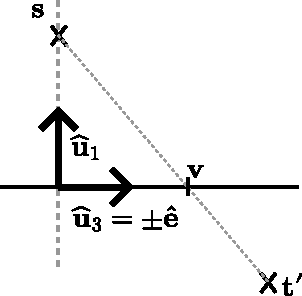
\includegraphics[width=0.5\textwidth]{figures/annex-first-order-diffraction-2.pdf}
        \caption{View in the plane $\LB \ov, \widehat{\uv}_1, \widehat{\ev} \RB$, containing $\sv$, the edge, and the rotated target $\tv'$.}
        \label{fig:diffraction-first-order-b}
    \end{subfigure}
    \caption{Illustration of rotating the target $\tv$ about the edge $\widehat{\ev}$ by the angle $\phi$ to obtain the rotated target $\tv'$, which is coplanar with the source $\sv$ and the edge. The diffraction point $\vv$ is such that $\sv$, $\vv$, and $\tv'$ are collinear.}
    \label{fig:diffraction-first-order}
\end{figure}

Minimizing $\Lc\LB x \RB$ with the rotated target $\tv'$ is equivalent to $\sv$, $\vv$, and $\tv'$ being collinear, i.e.
\begin{align}
    (\vv - \sv) \times \overrightarrow{\sv\tv'} &= \zerov \\
    \Leftrightarrow\quad x \left( \widehat{\ev} \times \overrightarrow{\sv\tv'} \right) &= \sv \times \overrightarrow{\sv\tv'}
\end{align}
where $\overrightarrow{\sv\tv'} = \tv' - \sv$.
Since $\widehat{\ev} \times \overrightarrow{\sv\tv'}$ and $\sv \times \overrightarrow{\sv\tv'}$ are parallel, the solution for $x$ is
\begin{equation}
    x = \operatorname{sign} \left( \left[ \widehat{\ev} \times \overrightarrow{\sv\tv'} \right]\tp \left[\sv \times \overrightarrow{\sv\tv'}\right] \right)
    \frac{ \norm{ \sv \times \overrightarrow{\sv\tv'} } }
         { \norm{ \widehat{\ev} \times \overrightarrow{\sv\tv'} } }.
\end{equation}